\chapter{Methodology}
\label{chap:2}
\ChapterPageStuff{2}

\section{Preamble}
In this chapter the methodology to create and implement a logging mechanism to do system utilisation analysis on software system will be discussed. In \Cref{sec:EventLogging} provided the needed literature to create a logging mechanism in \Cref{sec:Ch3_LoggingMechanism} for two software systems.

\section{Logging mechanism}\label{sec:Ch3_LoggingMechanism}
For this study two software systems are used to implement the logging mechanism. The first software system which will be called System A, is energy management system that uses combination of PHP and \textit{.NET Framework}\footnote{\label{ftn:NetFramework}\textbf{.NET Framework} is a run-time execution environment that consists of common language run-time (CLR) and a .NET Framework Class Library \cite{Harkness2007}.} with a MVC architecture. System A will need to make use of two logging mechanism to log all the needed data of the activities of the user.\par System B is a \textit{.NET Framework}\footref{ftn:NetFramework} system with a MVC architecture and is the administrative software system to configure System A.

\begin{figure}[!htb] % An h :here, t: top, b: bottom.
	\centering % cent the figure
	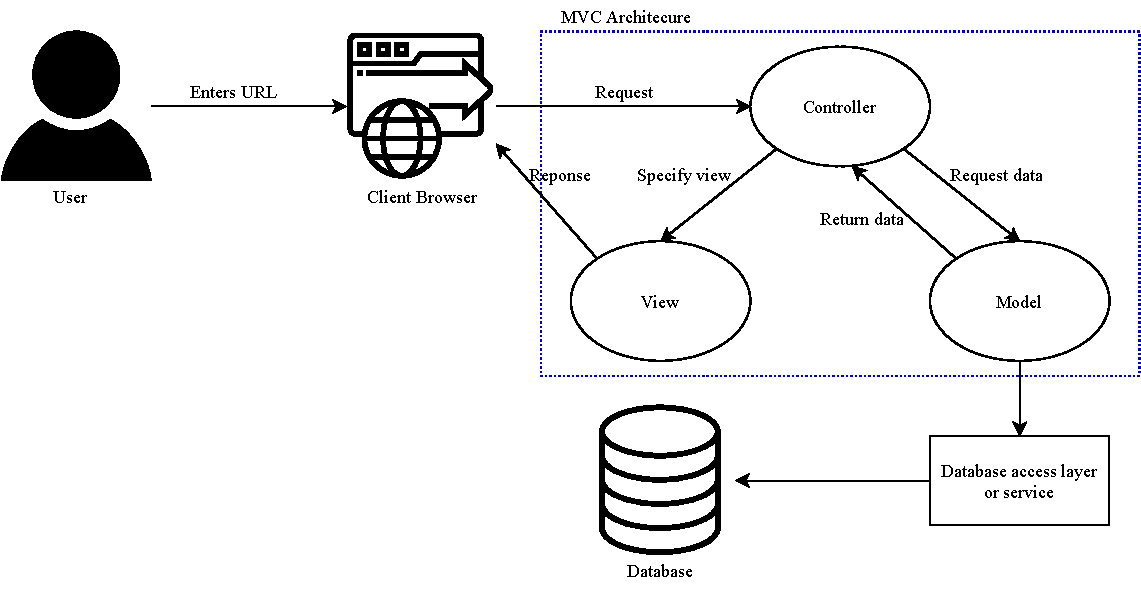
\includegraphics[width=0.95\textwidth]{Images/Chapter2/Flow_MVC_Architecture/Flow_MVC_Architecture.pdf}
	\caption[Request flow in MVC architecture]
	{\textit{Request flow in MVC architecture \cite{Gu2010}}}\label{fig:Flow_MVC_Architecture}
\end{figure}

\subsection{Logging points}
Logging point are essential data that describes the event's key features when creating a log as discussed in \Cref{sec:Ch1_LoggignPoints}. Both System A and B have certain key logging points that needs to be obtained from the user generated event.

\subsubsection{System A's logging points}

\begin{table}[!htb]
	\centering
	\small
	\caption[Logging points]
	{\textit{PHP logging mechanism}}
	\label{tbl:PHP_LoggignMechanism}
	\begin{tabularx}{\textwidth}{|c|l|X|}
		\hline \textbf{Identification} & \textbf{Criteria} & \textbf{Description} \\
        \hline \textbf{lma\_ID} & Activity ID & The activity identification is a incremental number of the event that is logged.\\
        \hline \textbf{lma\_Time} & Activity timestamp & This is the time which the event took place.\\
		\hline \textbf{lma\_d\_ID} & Dashboard ID & Foreign reference key to the Dashboard table.\\
		\hline \textbf{lma\_File} & File origin & \\
		\hline
	\end{tabularx}
\end{table}

\begin{figure}[!htb] % An h :here, t: top, b: bottom.
	\centering % cent the figure
	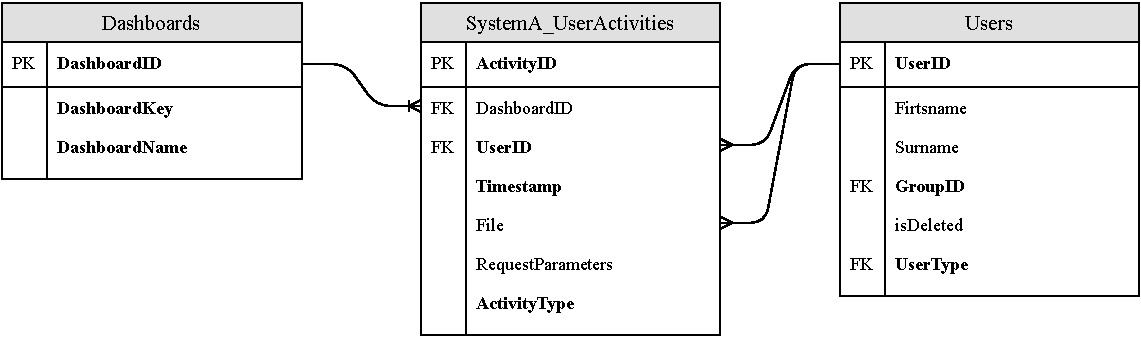
\includegraphics[width=0.95\textwidth]{Images/Chapter2/SystemA_ERD_Basic/SystemA_ERD_Basic.pdf}
	\caption[System A user activity ERD]
	{\textit{System A user activity ERD}}\label{fig:SystemA_Basic_ERD}
\end{figure}

\subsection{System A logging mechanism design}

In \Cref{fig:SystemA_Arch_Design} is the design for the System A's logging mechanism that consist of two different operations two log the event data that is generated from the user. These two main operations are used based on where the event is generated from either the PHP or MVC software components. The logging mechanism consist of two main functional requirements (\textbf{F/R}) that two main operations will use.

\begin{figure}[!htb] % An h :here, t: top, b: bottom.
	\centering % cent the figure
	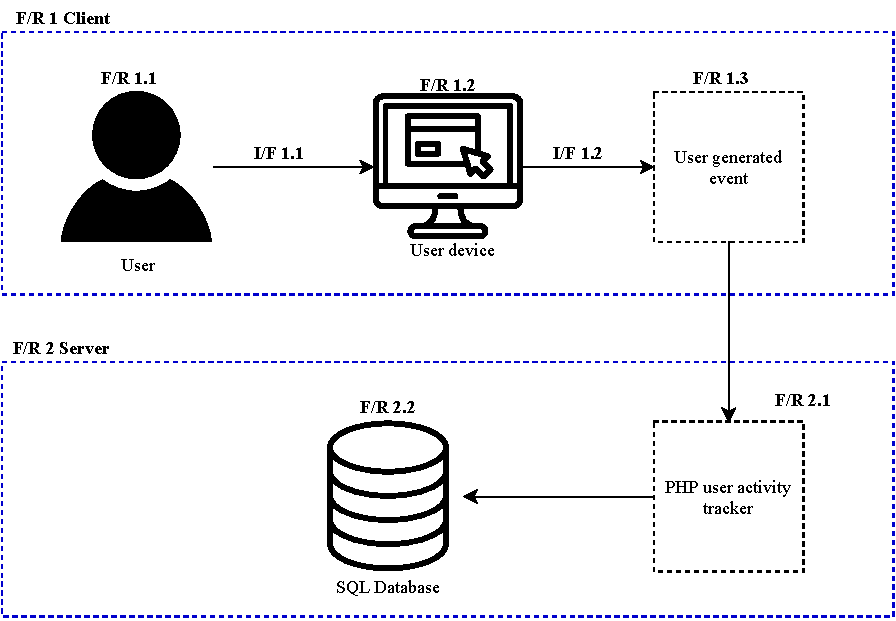
\includegraphics[width=0.99\textwidth]{Images/Chapter2/SystemA_Architecture_Diagram/SystemA_Architecture_Diagram.pdf}
	\caption[System A logging mechanism architecture design]
	{\textit{System A logging mechanism architecture design}}\label{fig:SystemA_Arch_Design}
\end{figure}

\textbf{F/R 1} of \Cref{fig:SystemA_Arch_Design} is the client side of the logging mechanism of System A.

\begin{table}[!htb]
	\centering
	\small
	\caption[System A's logging mechanism sub-systems]
	{\textit{System A's logging mechanism sub-systems}}
	\label{tbl:SystemA_SubSystems}
	\begin{tabularx}{\textwidth}{|l|X|}
		\hline \textbf{F/R 1.1} & The user \\
		\hline
	\end{tabularx}
\end{table}

\clearpage

\begin{figure}[!htb] % An h :here, t: top, b: bottom.
	\centering % cent the figure
	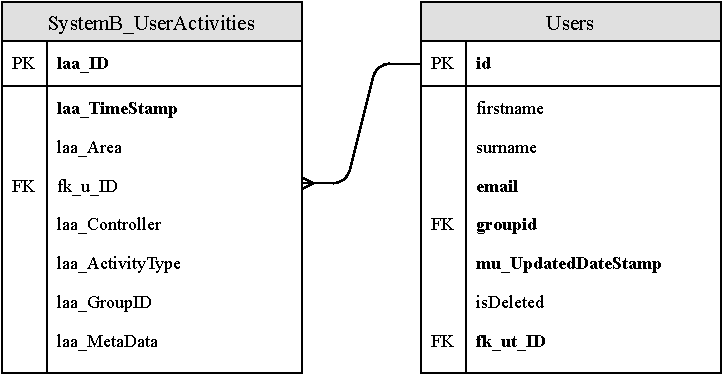
\includegraphics[width=0.6\textwidth]{Images/Chapter2/SystemB_ERD_Basic/SystemB_ERD_Basic.pdf}
	\caption[System B user activity ERD]
	{\textit{System B user activity ERD}}\label{fig:SystemB_Basic_ERD}
\end{figure}

\subsection{Logging mechanism}

\section{System utilisation analysis}

\section{Integration}
In this section the integration of the utilisation analysis and logging mechanism will be discussed.

\section{Conclusion}
Conclude the chapter about the development of the logging mechanism and utilisation analysis.